%-*- coding: utf-8 -*-
\subsection{Composer plat}

L'analyse du cas d'utilisation composer un plat révèle quatre opérations : l'ajout, la modification, suppression et la consultation de plat. Se qui revient à définir les opérations CRUD (Create, Read, Delete, Update) pour la persistances des plats.

De plus, la solution doit respecter un modèle MVC.

Pour le modèle, les plats sont représenter par trois entités JPA : Plat, ComposantPlat, Ingrédient gérer par le framework Hibernate. L'entité ComposantPlat correspond à l'association d'un plat et d'un ingrédient et permet de stocker des informations comme la quantité d'un ingrédient dans un plat. De plus, chaque entité est géré par un DAO qui implémente les opérations CRUD.

Pour le contrôle, l'application utilise un servlet PlatServlet et un beans de contrôle PlatService.
La servlet est en charge de traiter les requête http GET et POST. Les requétes GET servent à envoyer le type d'opération à effectuer selon le format : /Plats\? action=[opération]\& id=[id du plat sur lequel porte l'action]. L'opération créer ne demande pas d'id, l'opération consulter sans id, revient à consulter tous les plats.
Les requêtes POST servent à envoyer les données servant à la création et à l'édition par le récupération des informations sur le plat dans un formulaire.
Le contrôleur traite les informations transmise à la servlet et modifie les entités selon l'opération demandé, elle a un durée de vie de type session et crée les DAO associé au entité.

La servlet redirige sur deux vue selon le type d'opération : consulterPlat.jsp pour les opérations consulter et supprimer, et editerPlat.jsp pour la création et l'édition. Chaque vue adapte son affichage en fonction du type d'opération. 

\begin{figure}
\centering
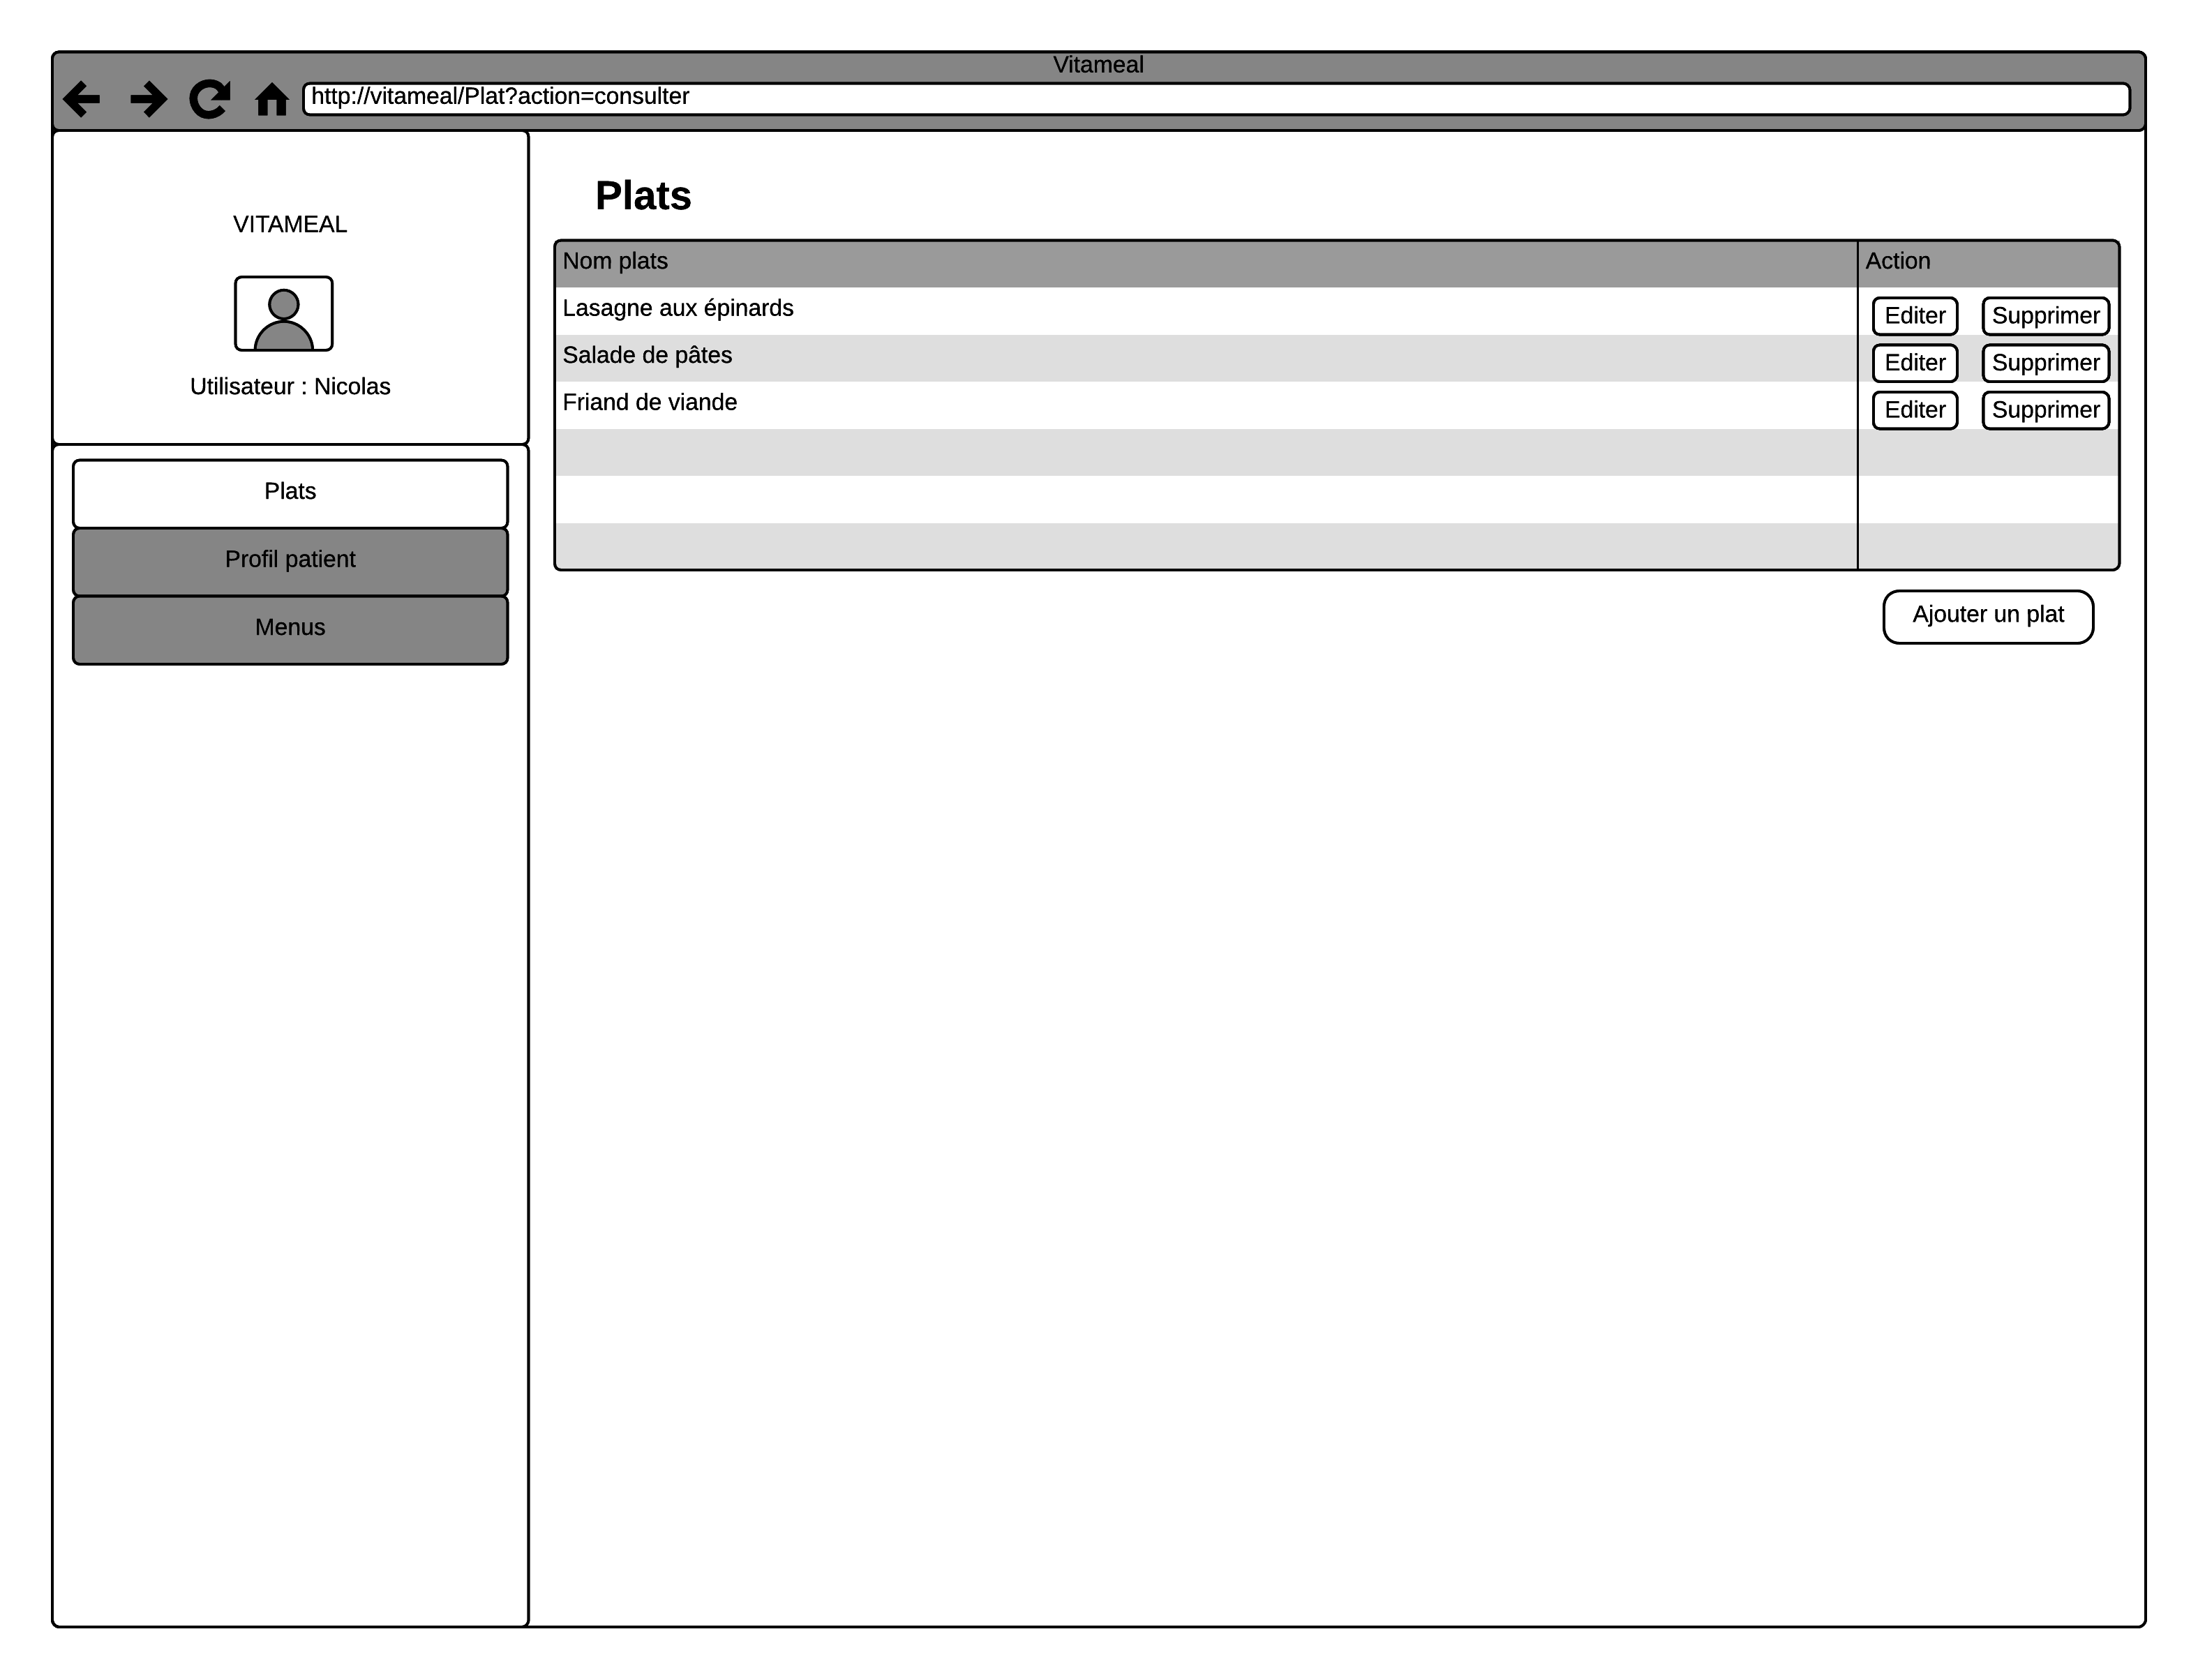
\includegraphics[scale=0.5]{../../CasDUtilisations/CompositionPlat/maquette_EcranConsulterPlats.png}
\caption{Maquette de consultation d'un plat}
\label{MaquetteConsultationPlat}
\end{figure}

\begin{figure}
\centering
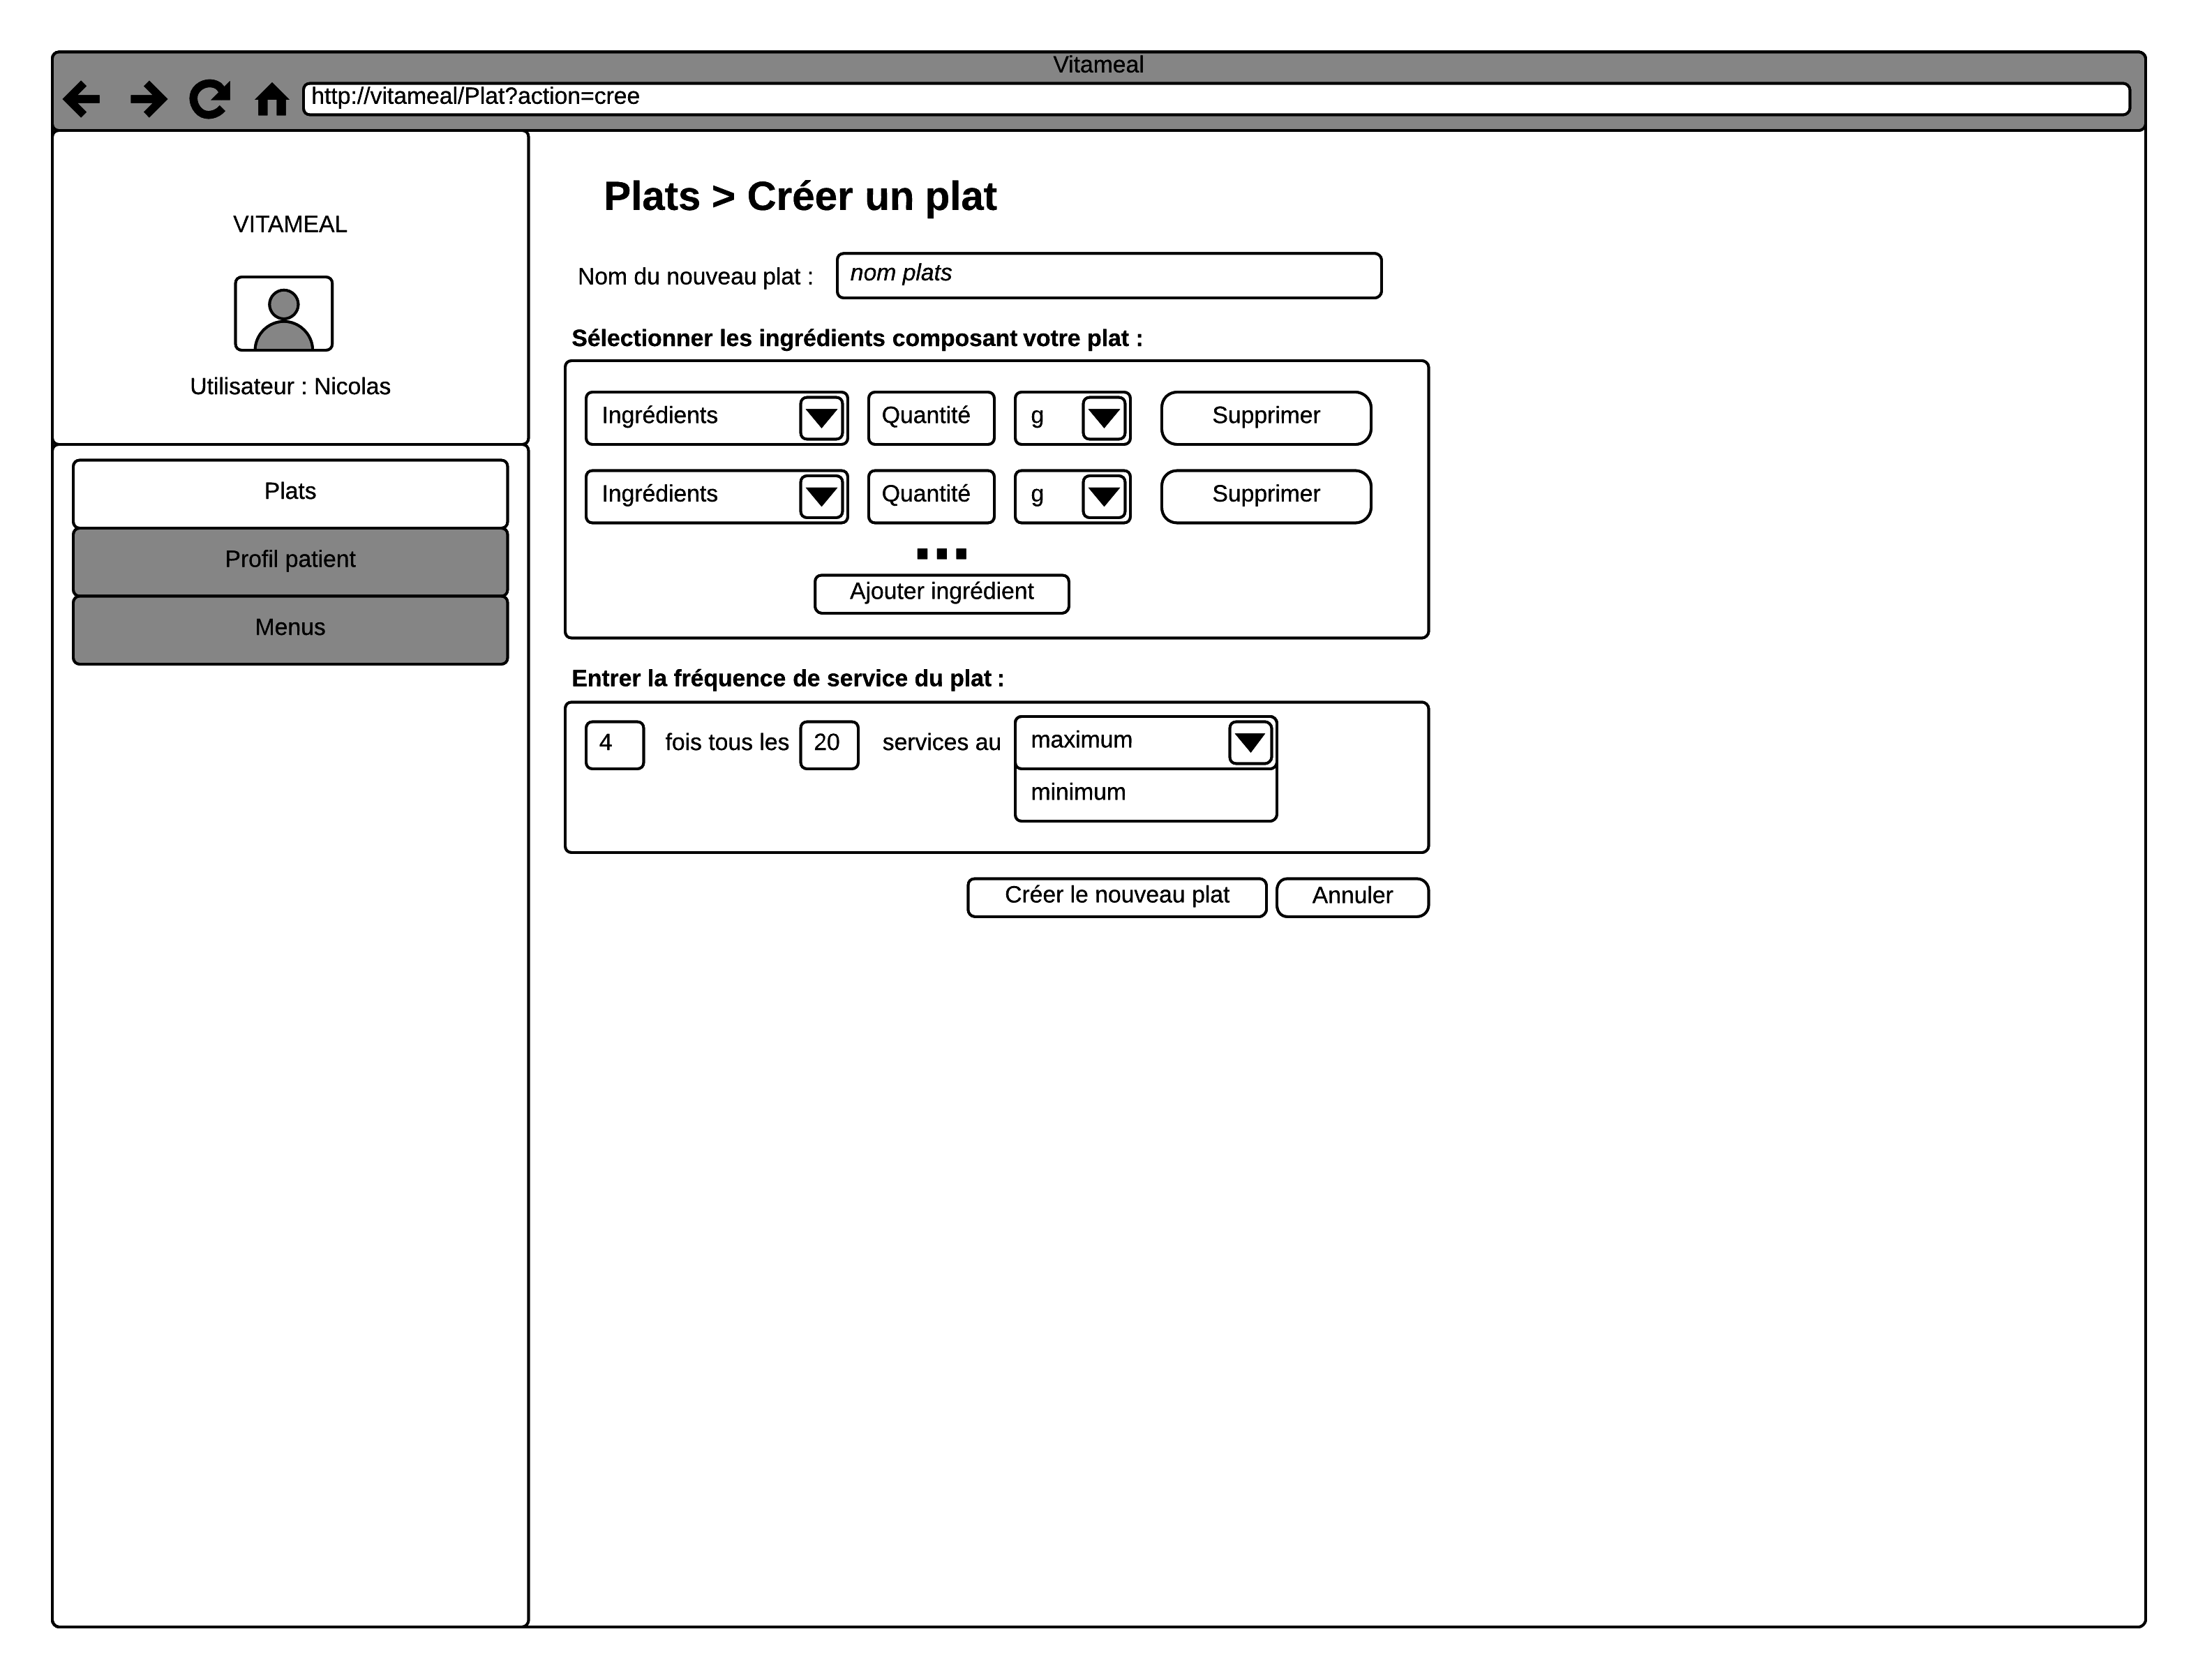
\includegraphics[scale=0.5]{../../CasDUtilisations/CompositionPlat/maquette_EcranCreationPlat.png}
\caption{Maquette de la création d'un plat}
\label{MaquetteCreationPlat}
\end{figure}

\begin{figure}
\centering
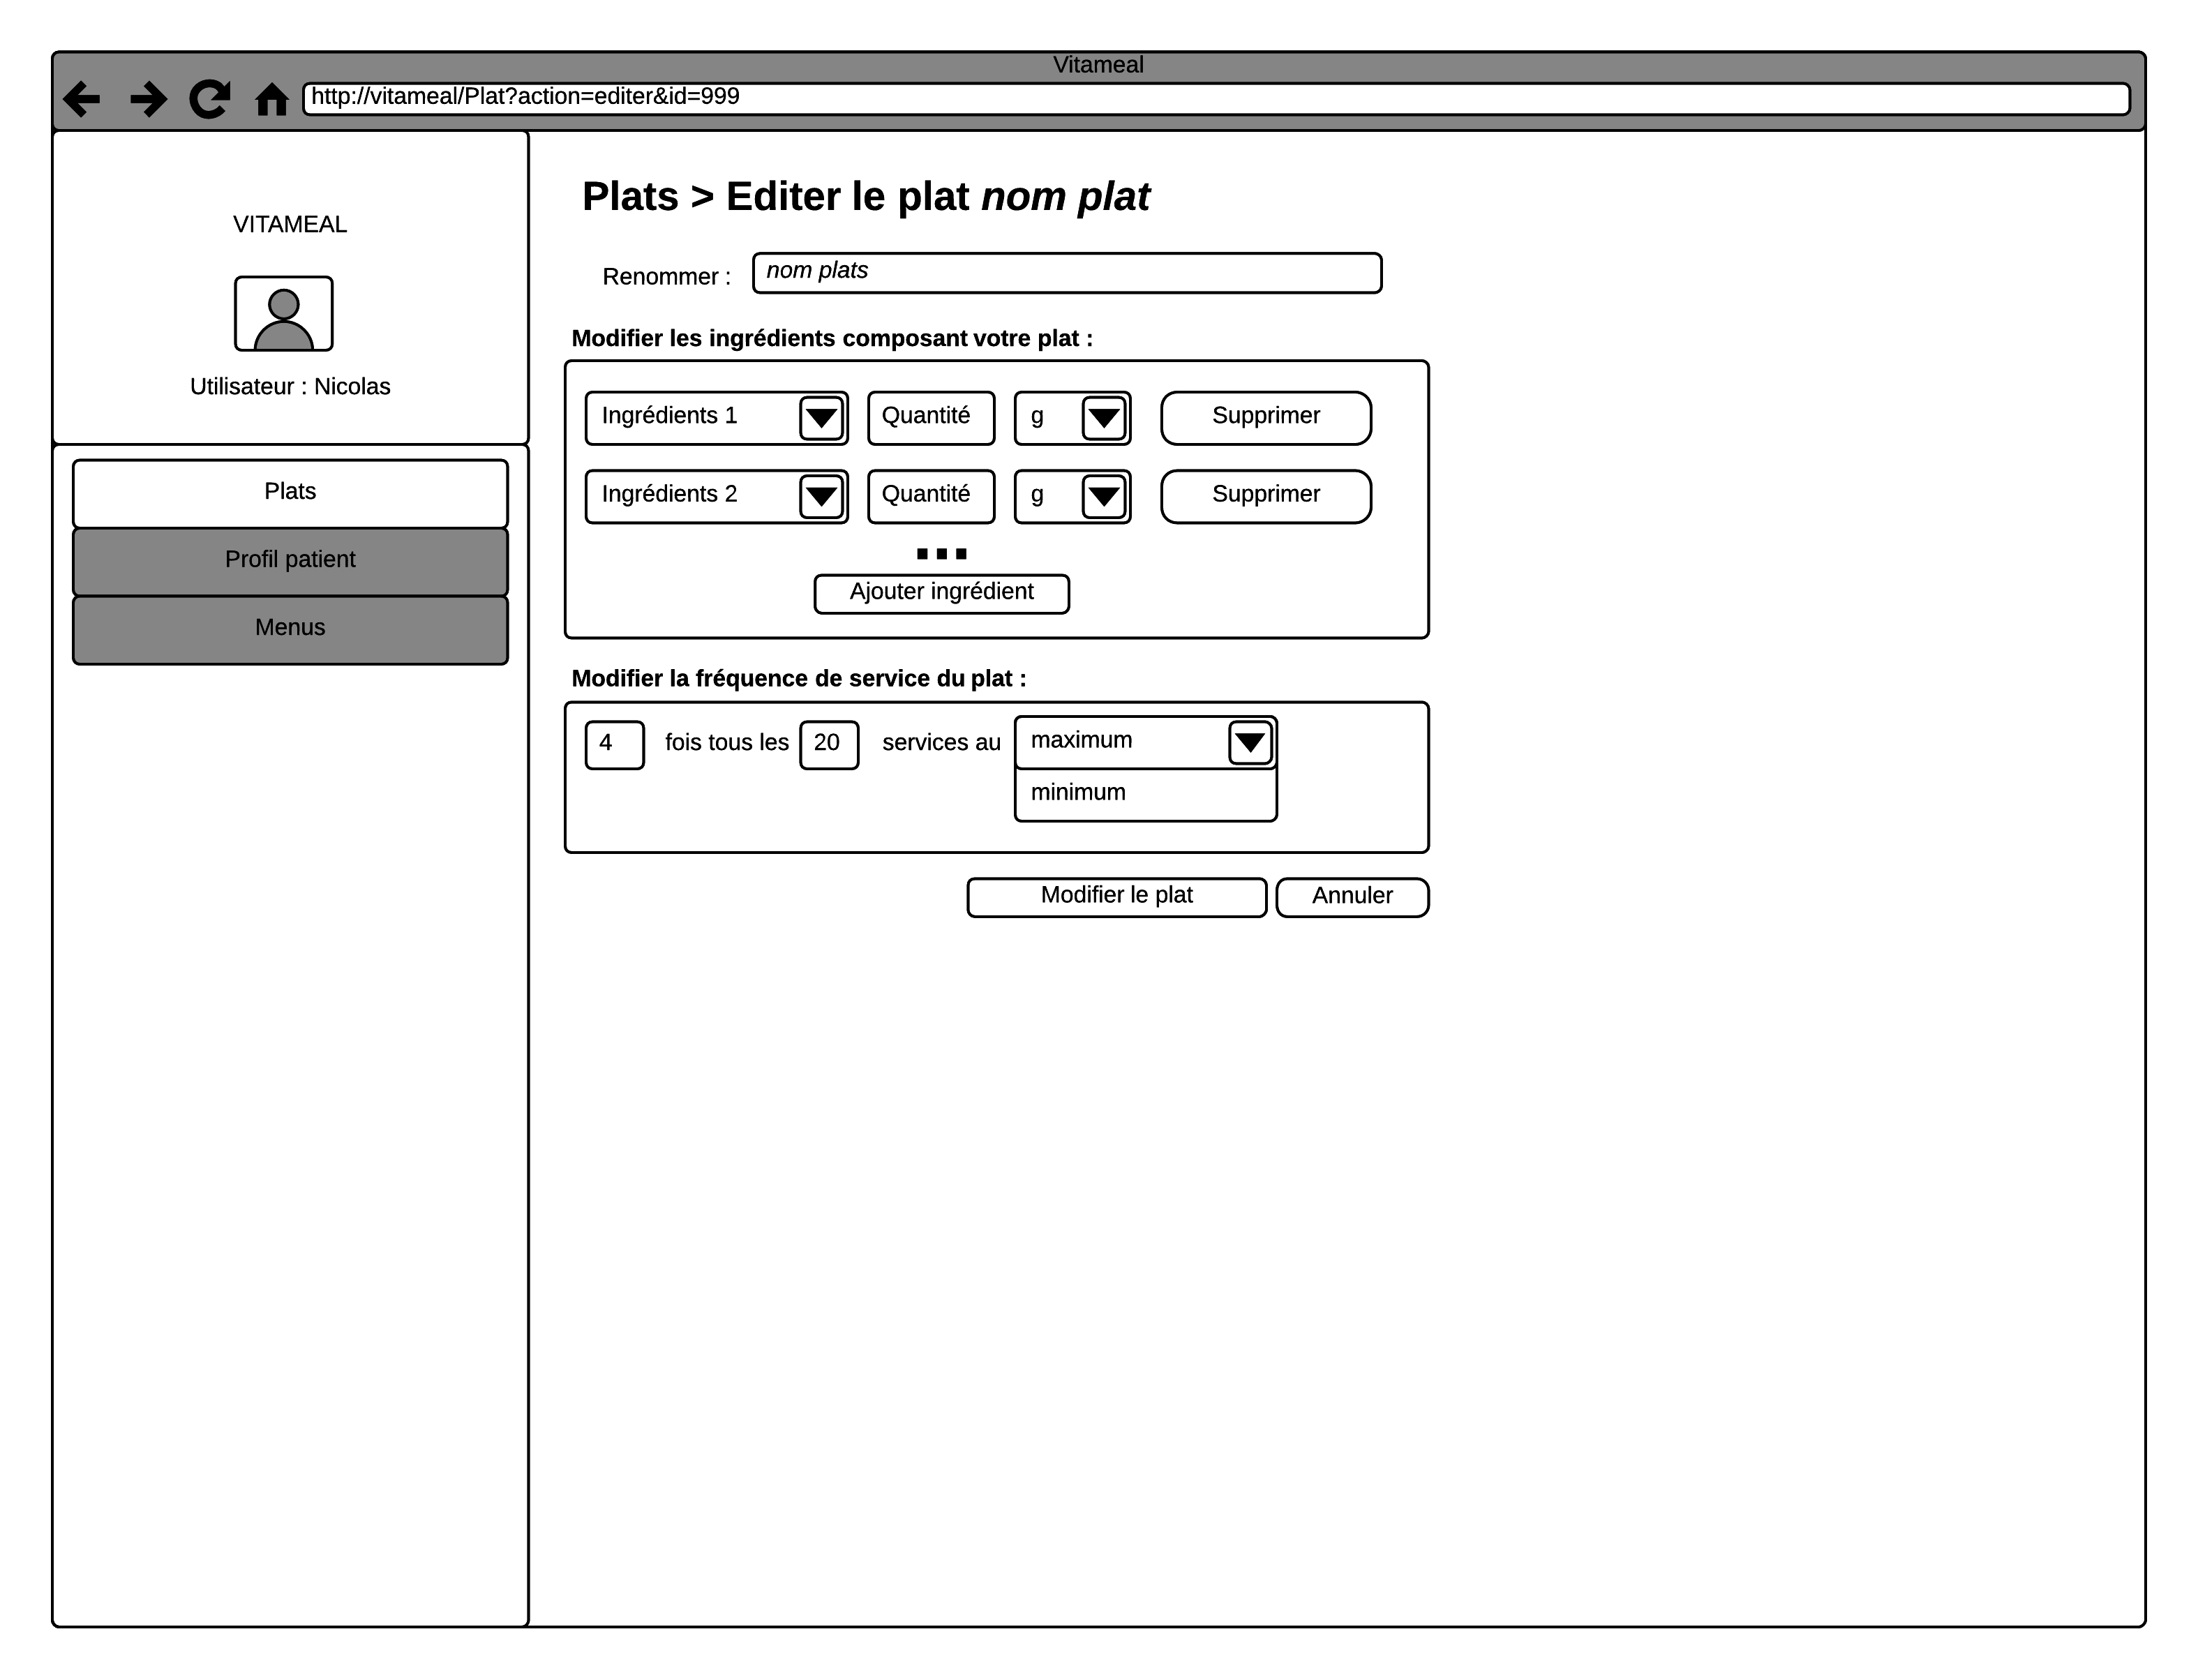
\includegraphics[scale=0.5]{../../CasDUtilisations/CompositionPlat/maquette_EcranEditionPlat.png}
\caption{Maquette de l'édition d'un plat}
\label{MaquetteEditionPlat}
\end{figure}

\begin{figure}
\centering
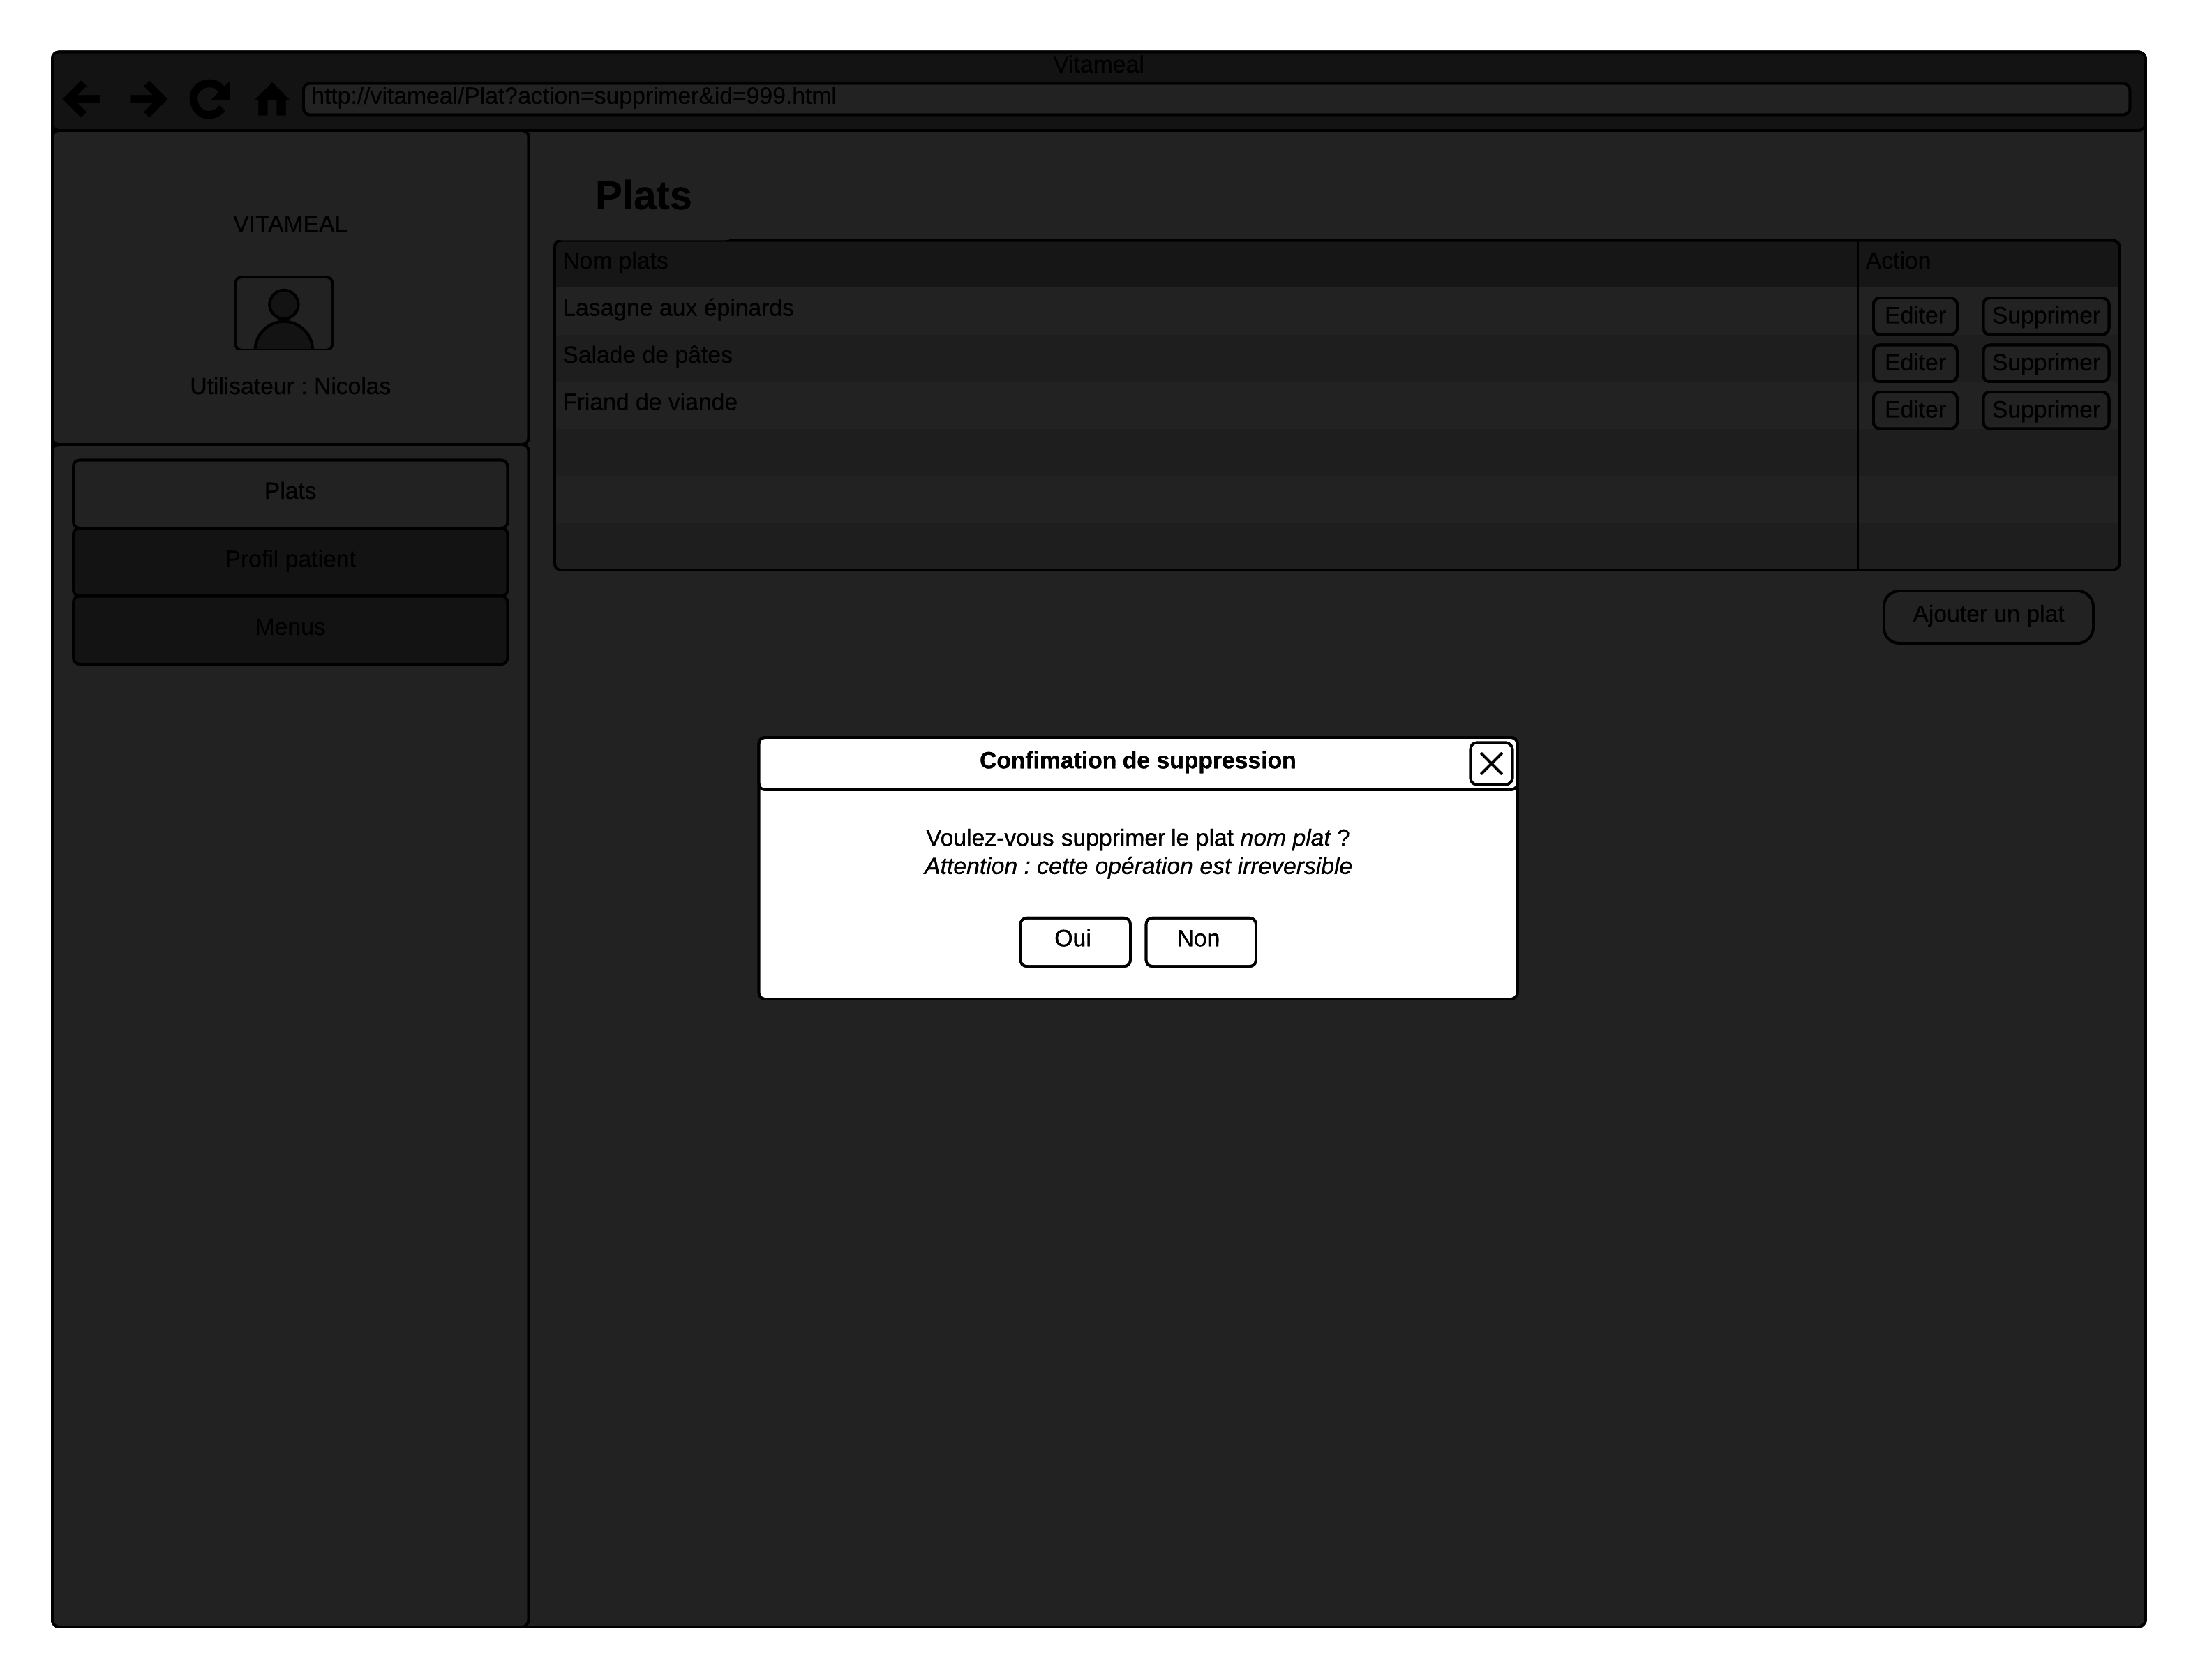
\includegraphics[scale=0.5]{../../CasDUtilisations/CompositionPlat/maquette_MessageSupressionPlat.png}
\caption{Maquette de suppression d'un plat}
\label{MaquetteSuppressionPlat}
\end{figure}

\begin{figure}
\centering
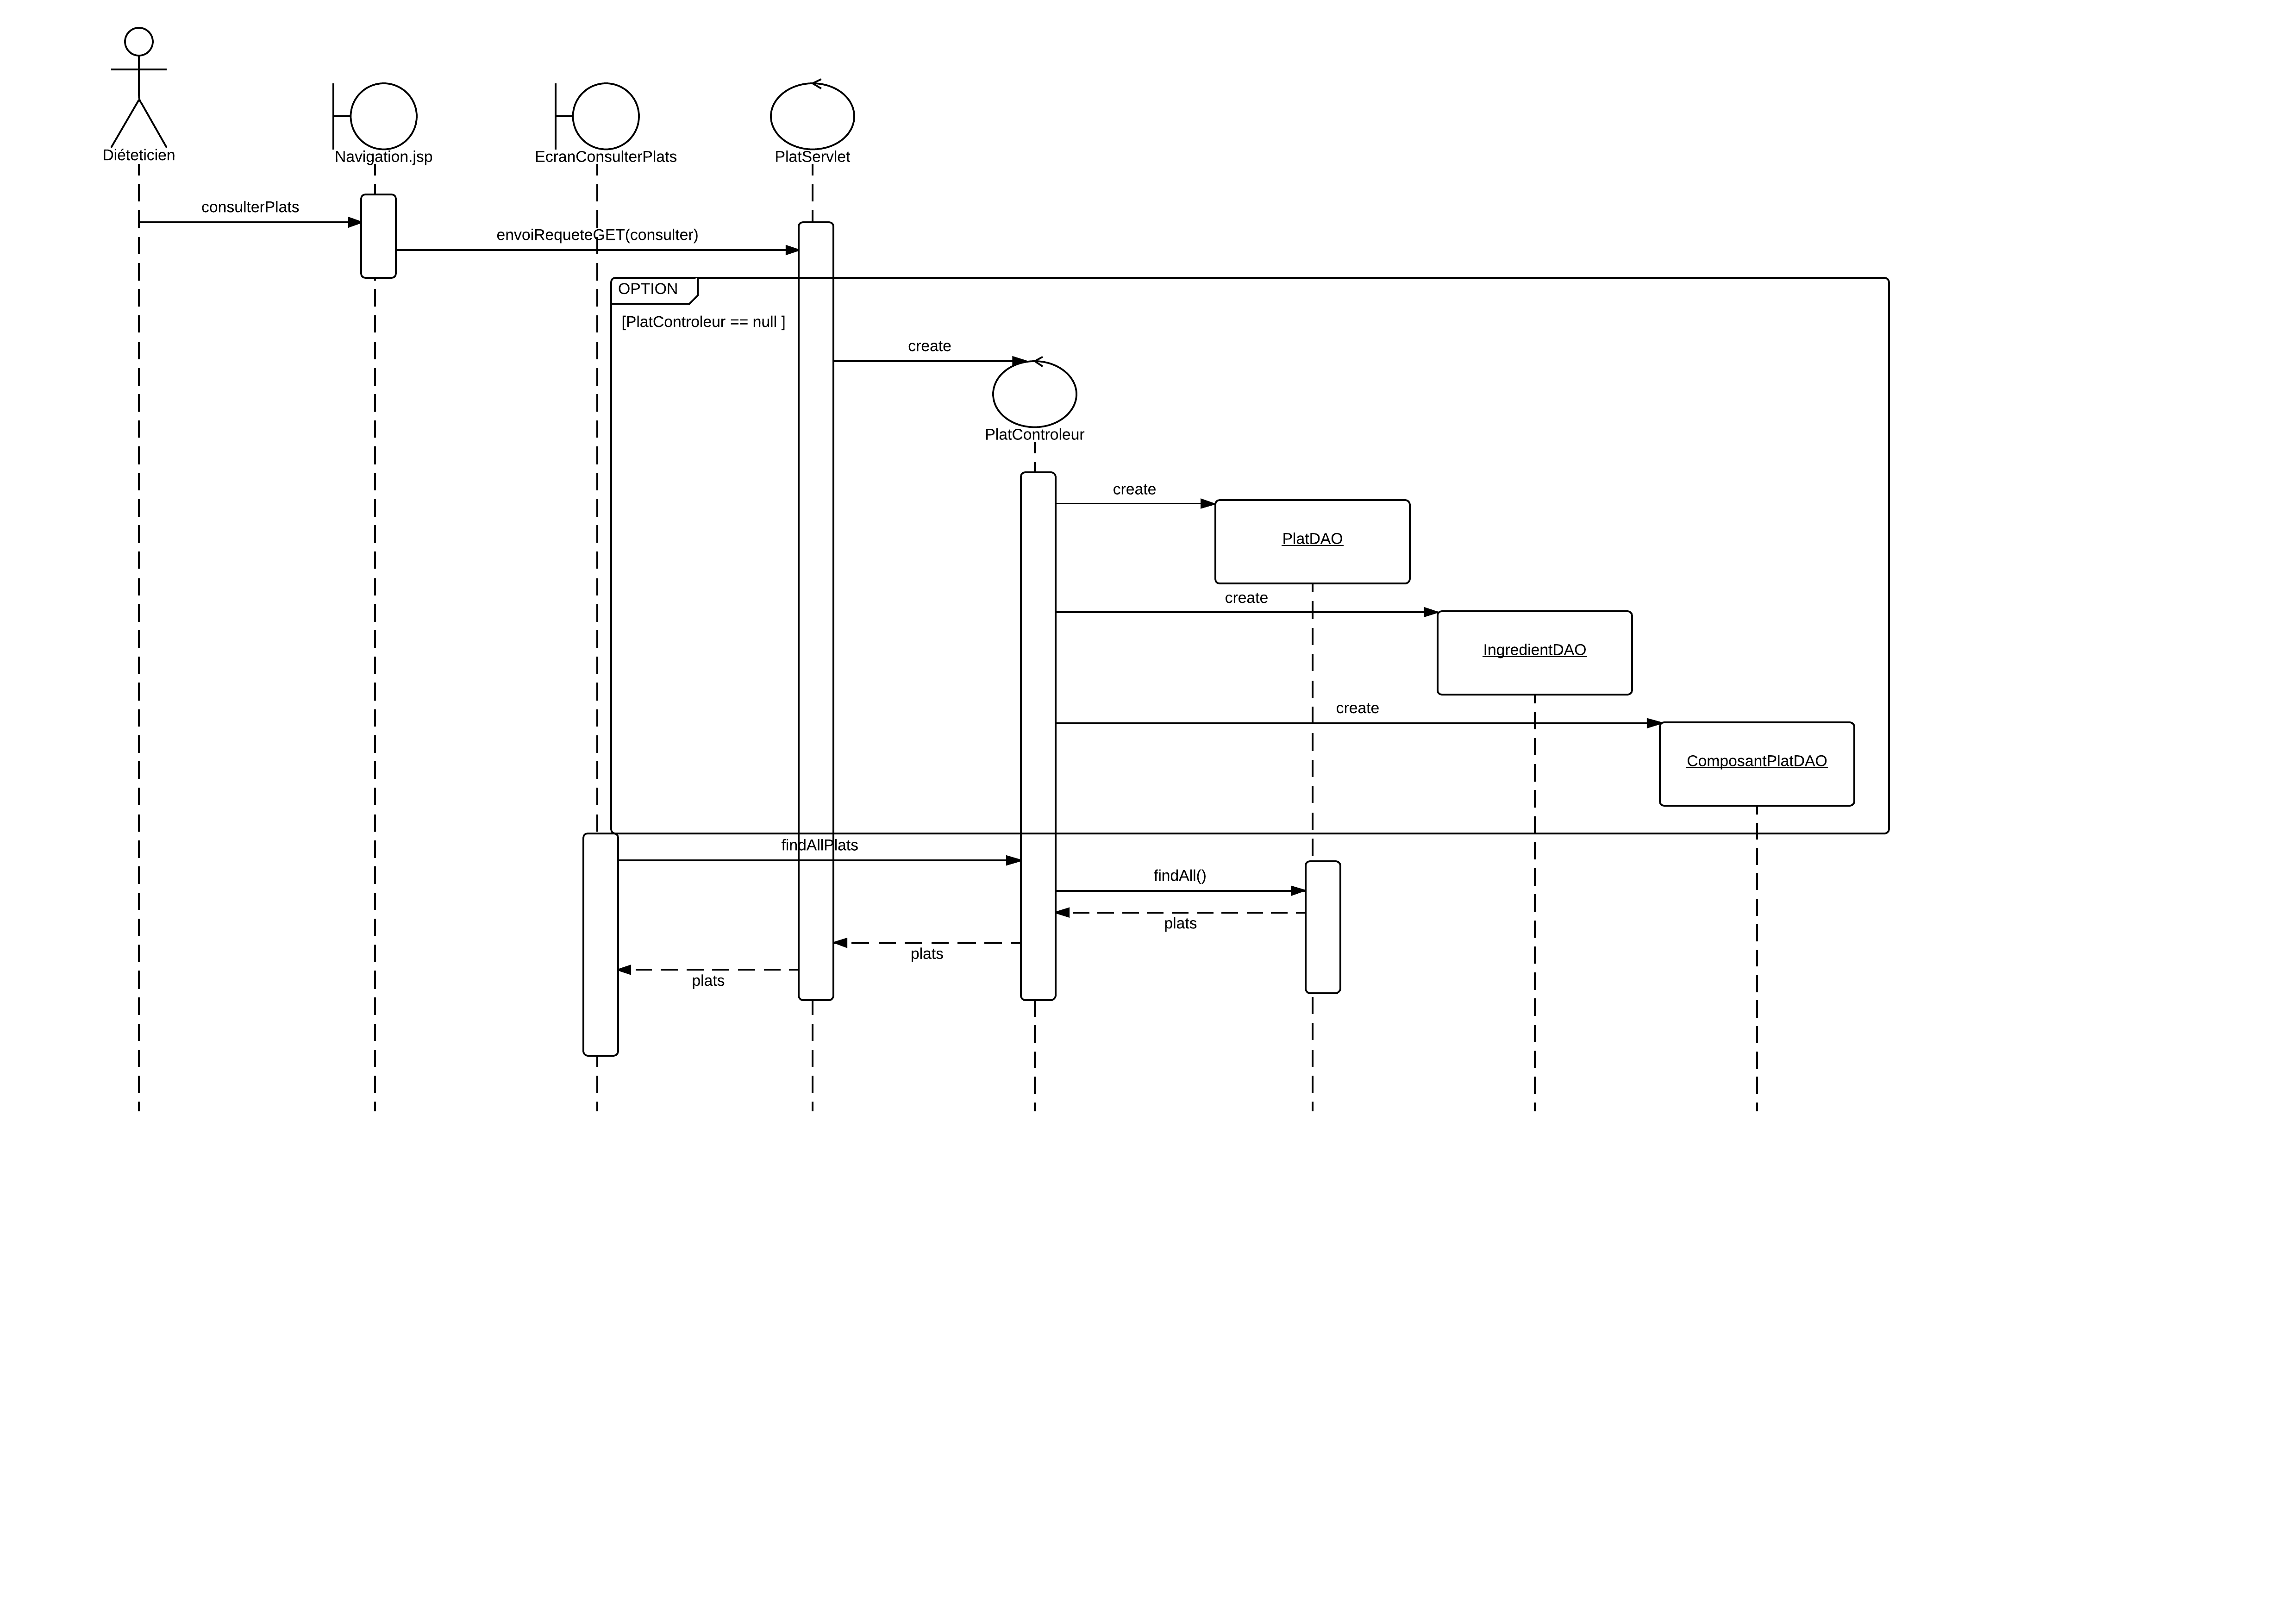
\includegraphics[scale=0.45]{../../CasDUtilisations/CompositionPlat/sequence_InitialisationPlatControleur.png}
\caption{Diagramme de séquence d'initialisation du contrôleur de plat}
\label{SequenceInitPlatControleur}
\end{figure}

\begin{figure}
\centering
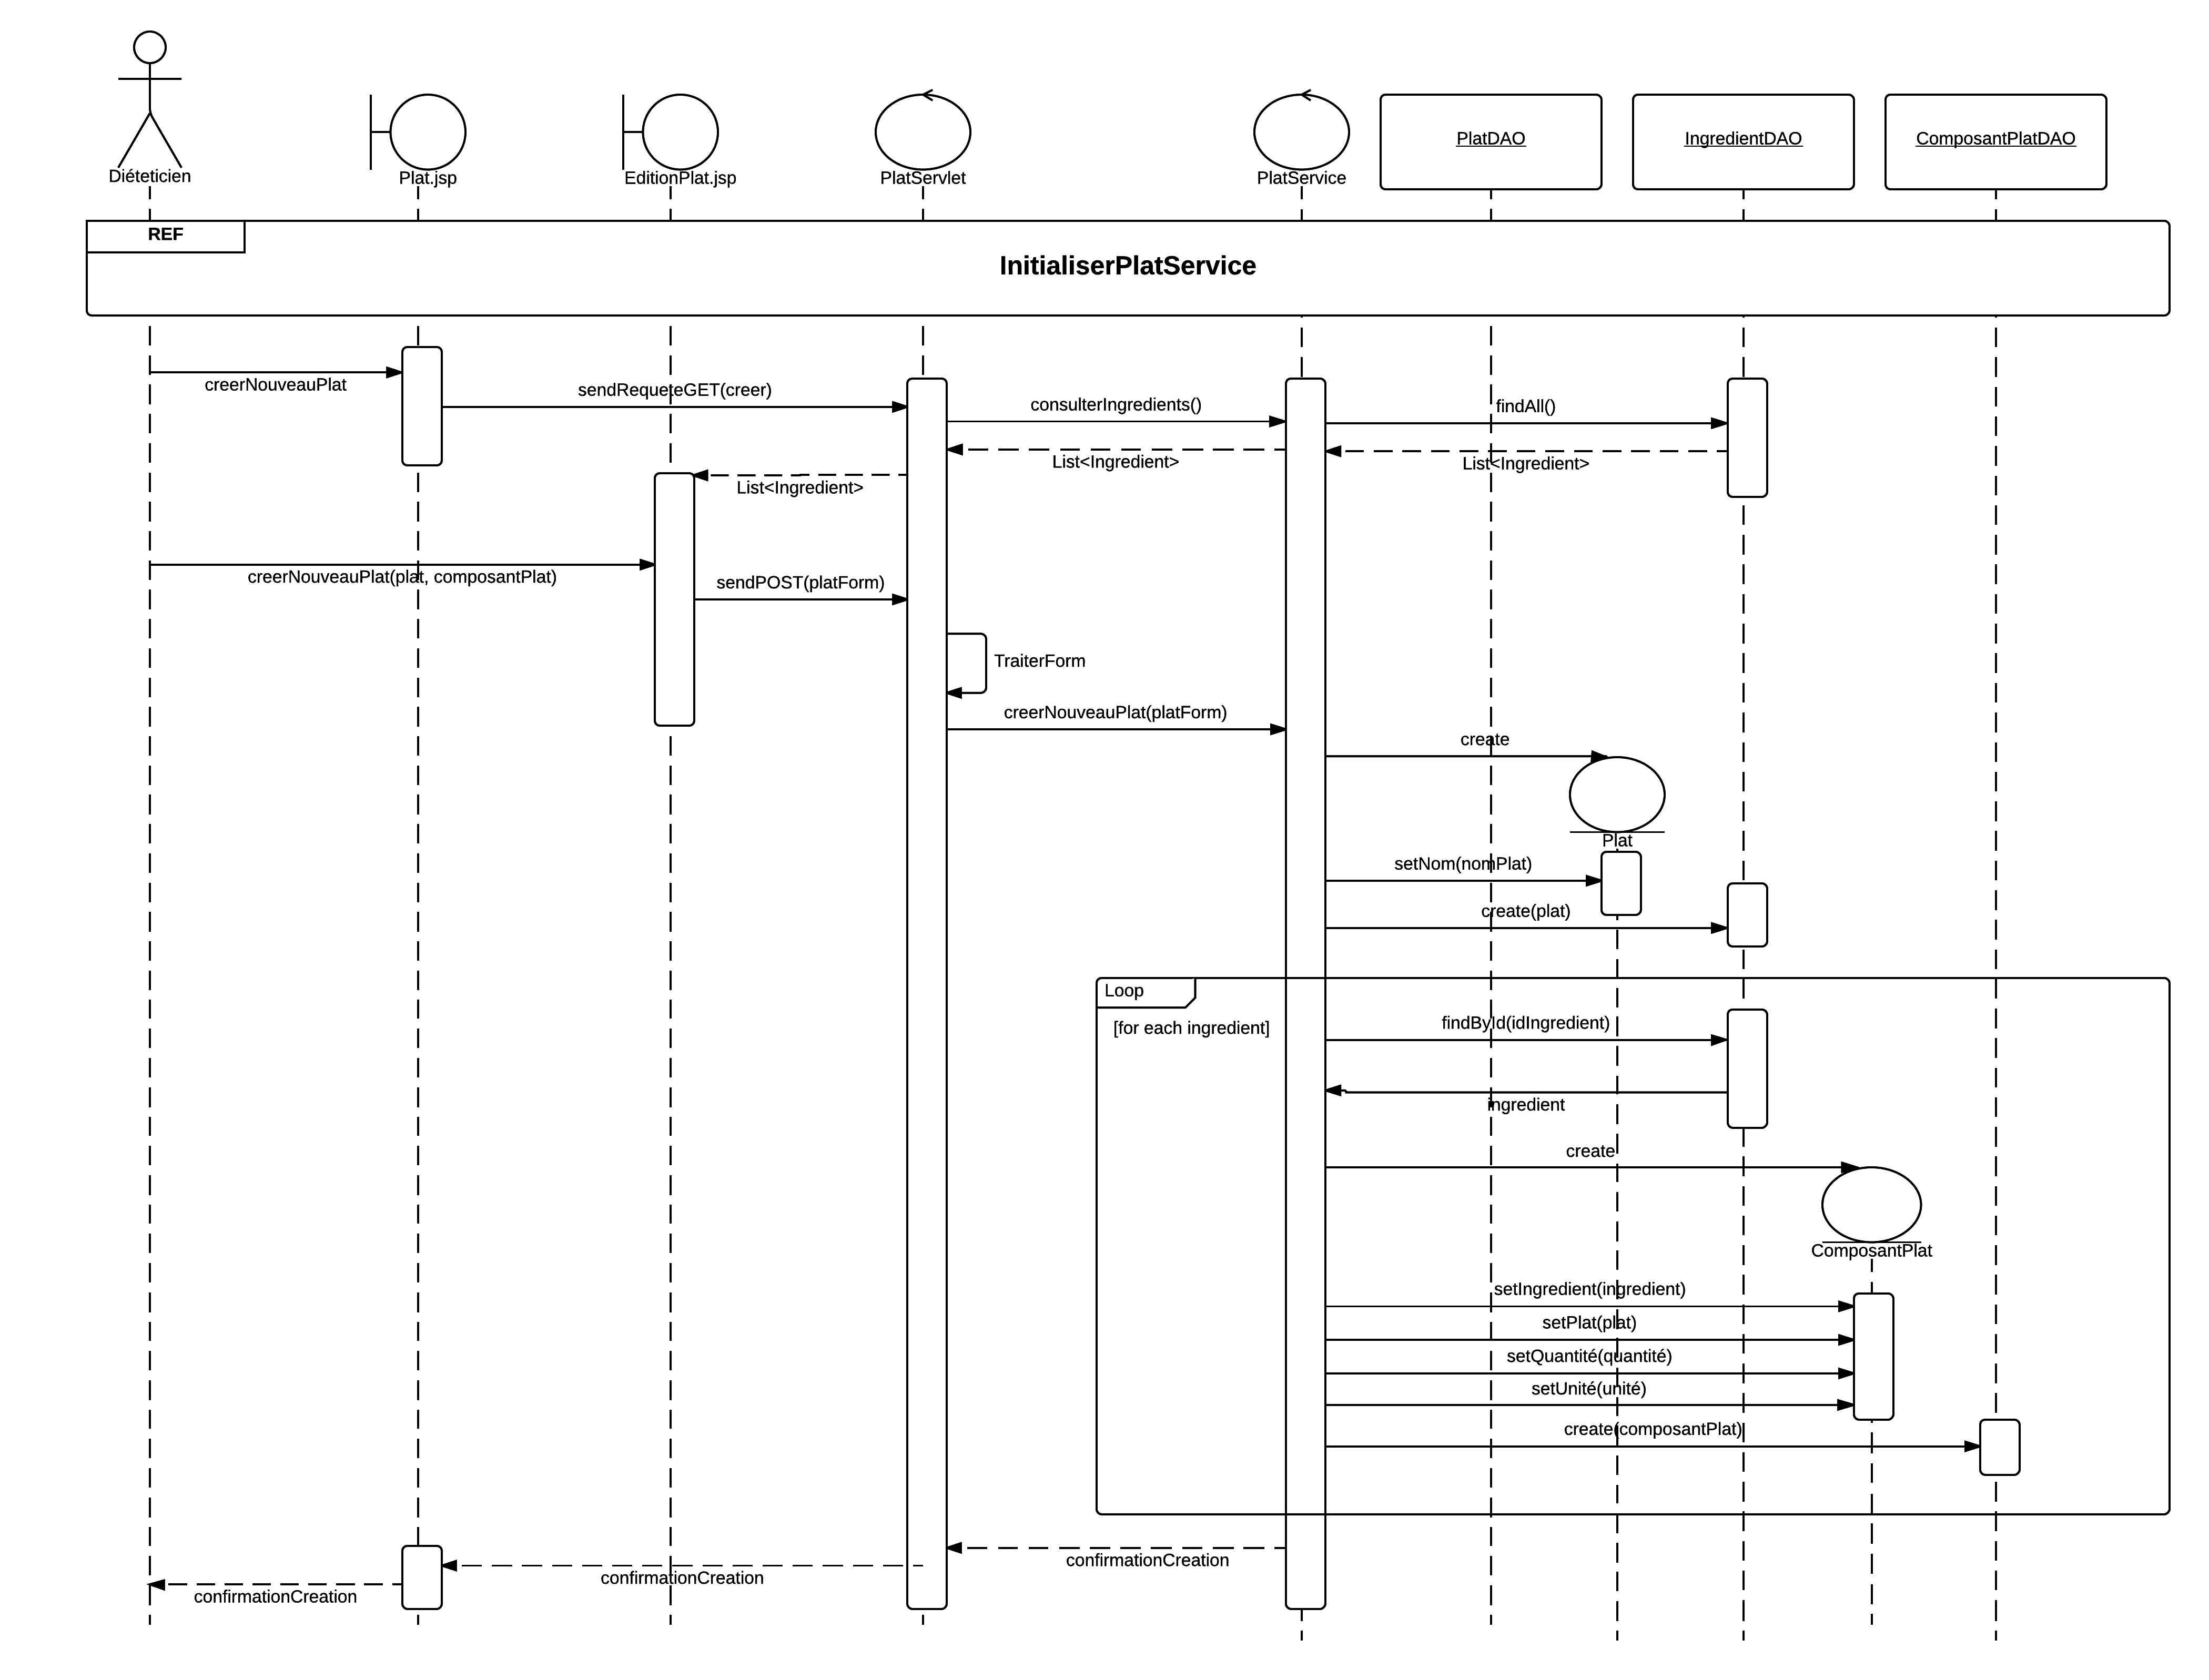
\includegraphics[scale=0.45]{../../CasDUtilisations/CompositionPlat/sequence_CreerPlat.png}
\caption{Diagramme de séquence de création d'un plat}
\label{SequenceCreerPlat}
\end{figure}

\begin{figure}
\centering
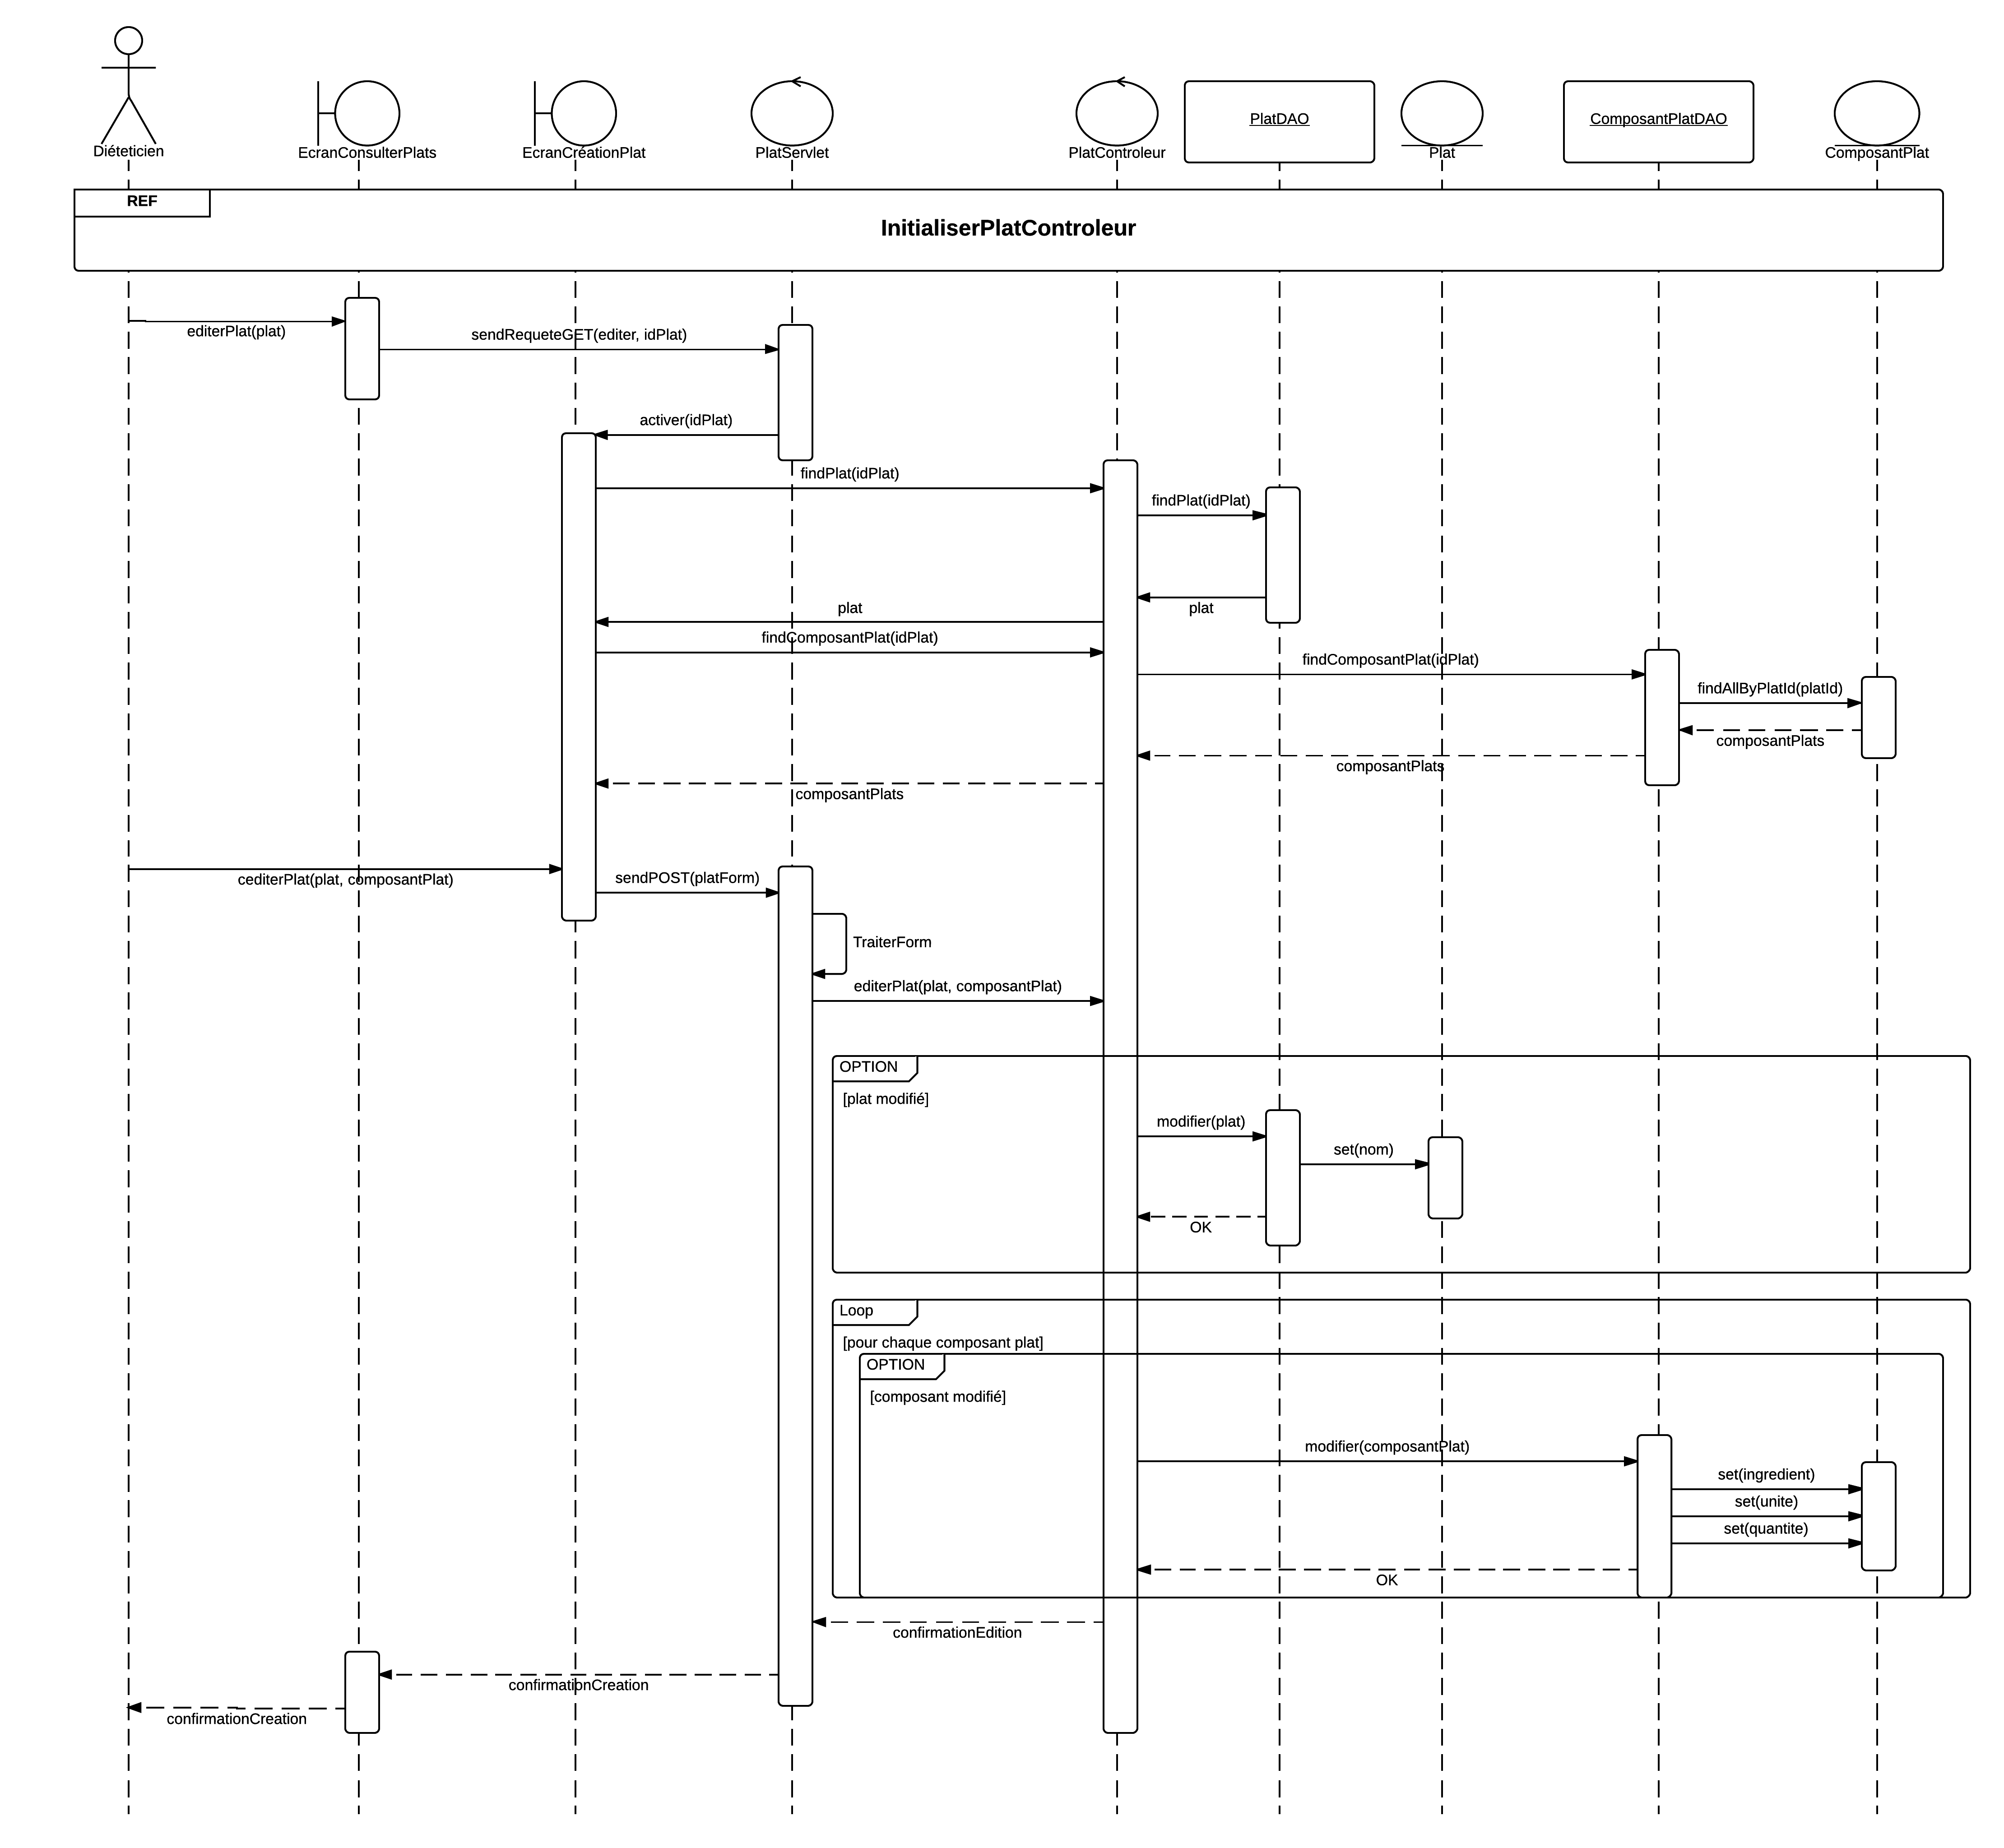
\includegraphics[scale=0.4]{../../CasDUtilisations/CompositionPlat/sequence_EditerPlat.png}
\caption{Diagramme de séquence d'édition d'un plat}
\label{SequenceEditerPlat}
\end{figure}

\begin{figure}
\centering
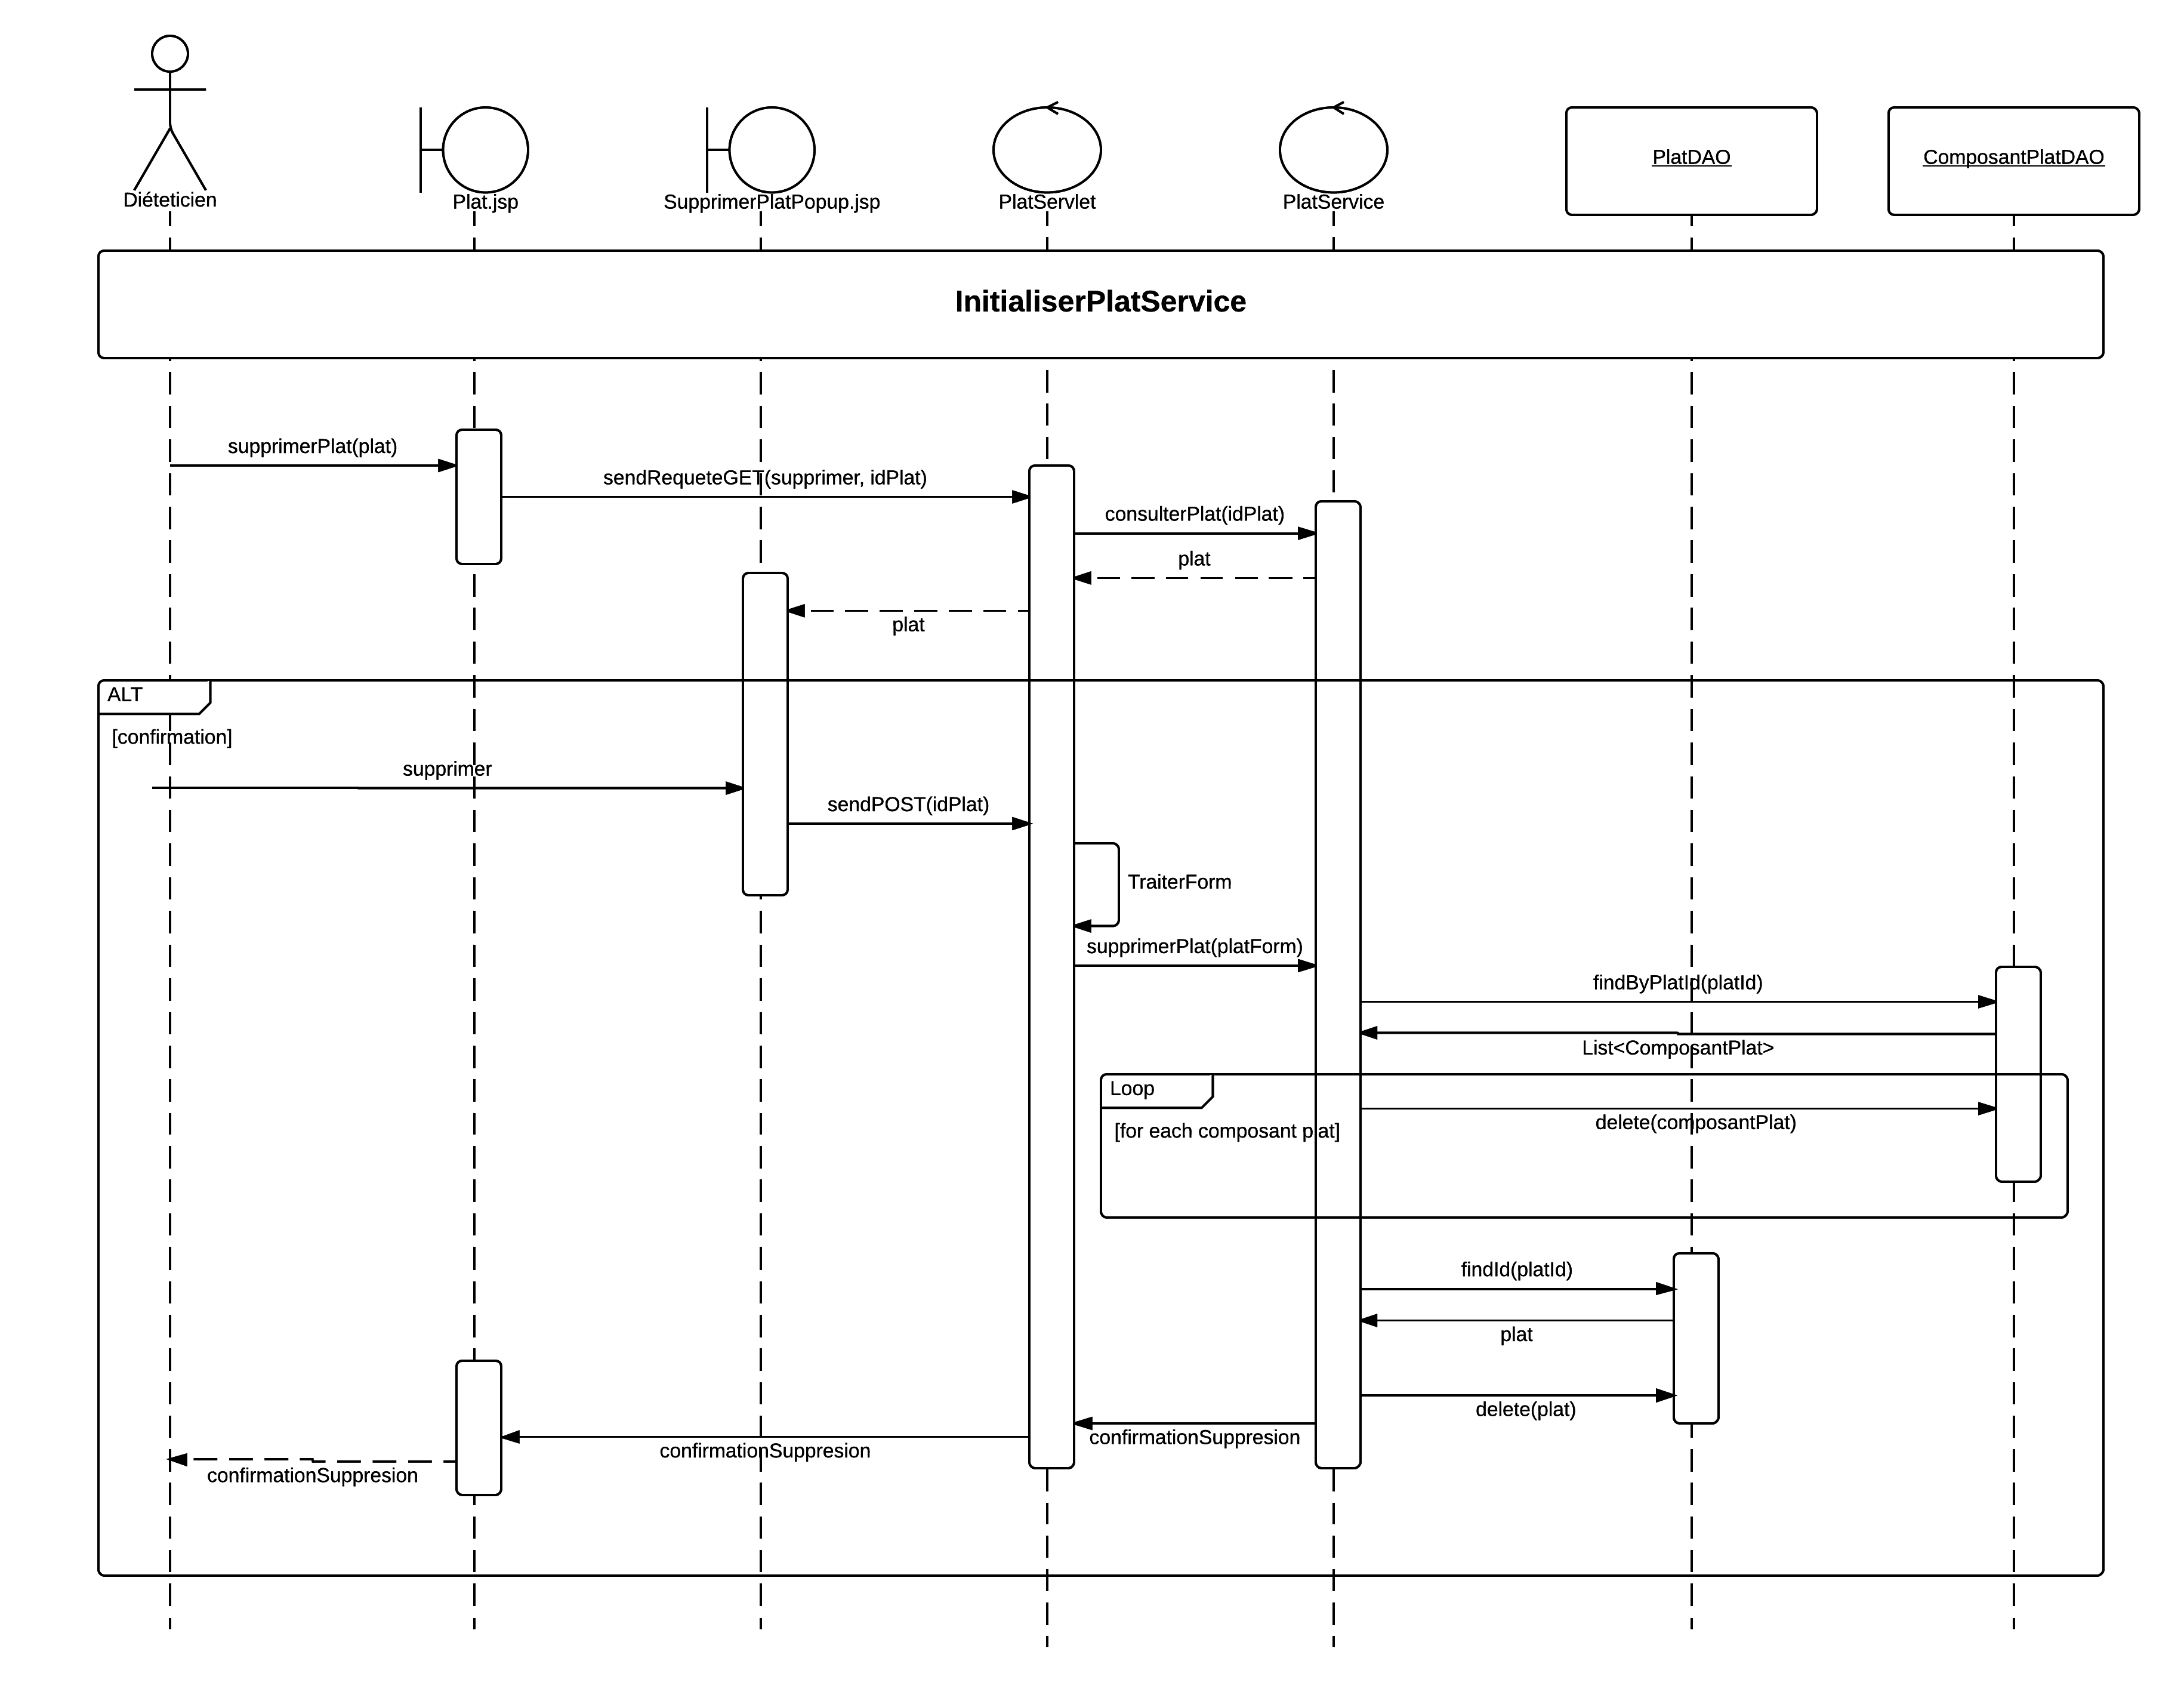
\includegraphics[scale=0.5]{../../CasDUtilisations/CompositionPlat/sequence_SupprimerPlat.png}
\caption{Diagramme de séquence de suppression d'un plat}
\label{SequenceSupprimerPlat}
\end{figure}

\begin{figure}
\centering
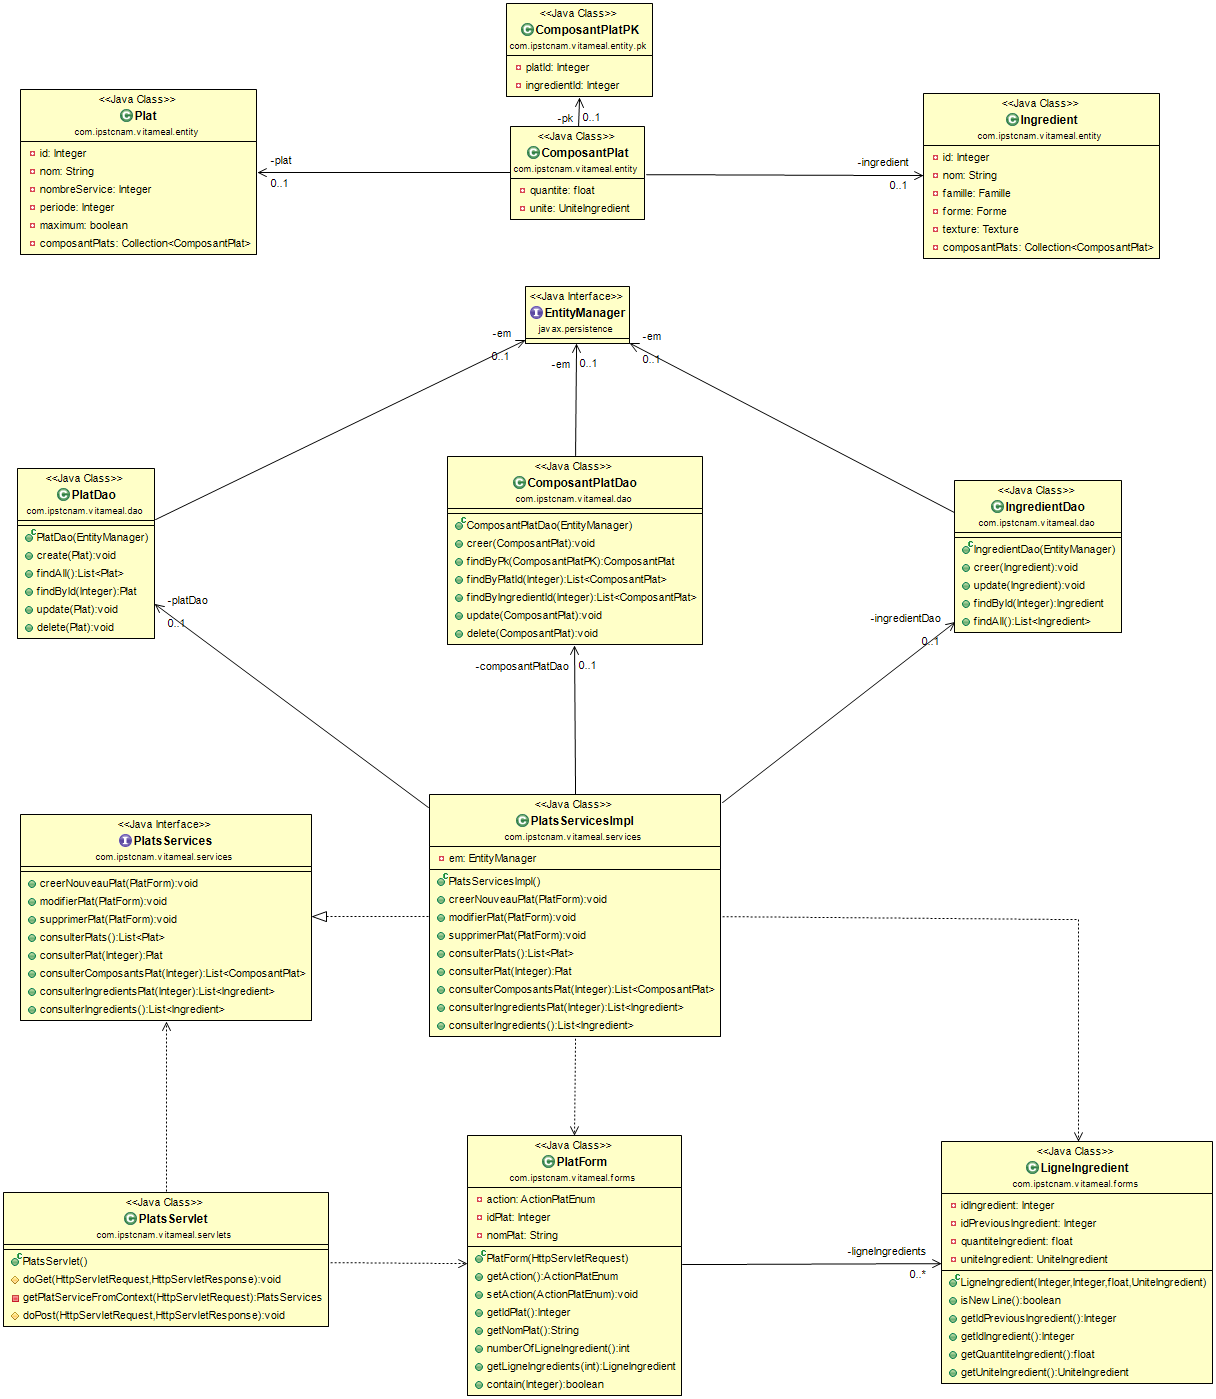
\includegraphics[scale=0.4]{../../CasDUtilisations/CompositionPlat/classDiagram_ComposerPlat.png}
\caption{Diagramme de classe de la compostion d'un plat}
\label{DiagrammeClassComposerPlat}
\end{figure}
